

\subsection{SPC evaluation}
\label{sec:eval_spc}
The evaluation section is now shifted to examine the images produced by the SPC. The images will be analyzed using the using a range of methods to examine the performance of the SPC. In this section the BRISQUE algorithm will be used again where connections to the previous result is drawn, a reconstructed image will be compared to an ideal image using homography, a set of images is presented reconstructed at different subsampling ratios, a edge response analysis i performed and the correlation between reconstruction performance and noise is conducted. 



\subsubsection{Image quality using no reference quality assessment}
In this section the blind quality assessment tool BRISQUE will be used to score the reconstructed images from the SPC. The same algorithm was used on the simulated data where a benchmark was set as a theoretical limit to the reconstructed images.\\[0.1in]     

Each image is evaluated at subsampling rate from $5\%$ to $30\%$ where the result is presented in figure~\ref{fig:brisque_plot}.

\begin{figure}[H]
    \centering
    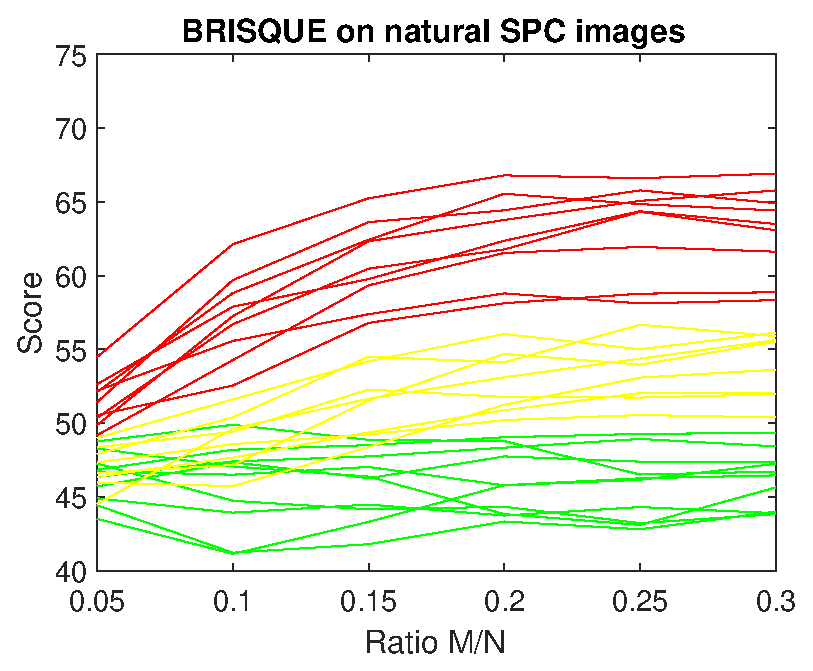
\includegraphics[width = 0.7\linewidth]{result/SPC_NRQA/brisque_spc.eps}
    \caption{BRISQUE score for images reconstructed from the SPC with subsampling ratios from $5\%$ to $30\%$. Each line represent one image and is classified with different colors representing start score at smallest subsampling ratio and general trend when subsampling ratio is increased.}
    \label{fig:brisque_plot}
\end{figure}


As seen in figure~\ref{fig:brisque_plot} each image as been plotted separately, this is because the high variance in the scores and the distinct different trends in the score. Furthermore the images has been classified into three different classes depending on the initial score at 5\% subsampling and the trend when increasing the subsampling ratio\todo{an visually inspecting the images}. The classes has been color coded where:

\begin{itemize}
\item Red means bad score from the first subsampling ratio and a trend line where the score gets worse with more samples.
\item Yellow represent good initial score but the trend line indicates worse image quality when subsampling ratio is increased.
\item Green represent both good initial score and better or stationary score when subsampling ratio is increased. 
\end{itemize}

When studying the BRISQUE score plot in figure~\ref{fig:brisque_plot} from the SPC and comparing to the plot of BRISQUE scores from simulated images in figure~\ref{fig:Brisque_2d} some similarities can be found. The first one is that, the best scores from the SPC has the same score as the simulated images with small or no noise added, which means that the SPC can compare to the benchmark set by the simulated images and thus gives theoretical optimal reconstruction given the measurement matrix and reconstruction algorithm. The second similarity is the trend of the "bad" images which has approximately the same score and trend as the simulated images with larger noise added to the sampled signal. In the last part of this subsection the reconstructed images will first be presented an analyzed followed by a noise analysis to conclude if there is a correlation between noise level and BRISQUE score.\\[0.1in] 


In figure~\ref{fig:good} to \ref{fig:bad} a sample of reconstructed  images are presented from each class with subsampling ratio 30\%. 




\begin{figure}[H]
    \centering
\begin{minipage}[t]{0.245\textwidth}
    \includegraphics[width=1\textwidth]{result/SPC_NRQA/g64_512_m30.PNG}
    \subcaption{}
    \label{fig:good1}
\end{minipage}
\begin{minipage}[t]{0.245\textwidth}
    \includegraphics[width = \textwidth]{result/SPC_NRQA/g24_512_m30.PNG}
    \subcaption{}
    \label{fig:good2}
\end{minipage}
\begin{minipage}[t]{0.245\textwidth}
    \includegraphics[width=1\textwidth]{result/SPC_NRQA/g22_512_m30.PNG}
    \subcaption{}
    \label{fig:good3}
\end{minipage}
\begin{minipage}[t]{0.245\textwidth}
    \includegraphics[width = \textwidth]{result/SPC_NRQA/g65_512_m30.PNG}
    \subcaption{}
    \label{fig:good4}
\end{minipage}
    \caption{Sample of "good" images corresponding to the green lines in figure~\ref{fig:brisque_plot}.
    (a) and (d) People sitting in the edge of a forest.  (b) Stationary car. (c) Camouflage jackets and a AT-4 anti-tank weapon on the ground.}
    \label{fig:good}
\end{figure}

\begin{figure}[H]
    \centering
\begin{minipage}[t]{0.245\textwidth}
    \includegraphics[width=1\textwidth]{result/SPC_NRQA/h35_512_m30.PNG}
    \subcaption{}
    \label{fig:half1}
\end{minipage}
\begin{minipage}[t]{0.245\textwidth}
    \includegraphics[width = \textwidth]{result/SPC_NRQA/h37_512_m30.PNG}
    \subcaption{}
    \label{fig:half2}
\end{minipage}
\begin{minipage}[t]{0.245\textwidth}
    \includegraphics[width=1\textwidth]{result/SPC_NRQA/h43_512_m30.PNG}
    \subcaption{}
    \label{fig:half3}
\end{minipage}
\begin{minipage}[t]{0.245\textwidth}
    \includegraphics[width = \textwidth]{result/SPC_NRQA/h62_512_m30.PNG}
    \subcaption{}
    \label{fig:half4}
\end{minipage}
    \caption{Sample of "medium good" images corresponding to the yellow lines in figure~\ref{fig:brisque_plot}.
    (a)  People sitting next to a parking lot. (b) - (d) House facades.}
    \label{fig:half}
\end{figure}

\begin{figure}[H]
    \centering
\begin{minipage}[t]{0.245\textwidth}
    \includegraphics[width=1\textwidth]{result/SPC_NRQA/b20_512_m30.PNG}
    \subcaption{}
    \label{fig:bad1}
\end{minipage}
\begin{minipage}[t]{0.245\textwidth}
    \includegraphics[width = \textwidth]{result/SPC_NRQA/b46_512_m30.PNG}
    \subcaption{}
    \label{fig:bad2}
\end{minipage}
\begin{minipage}[t]{0.245\textwidth}
    \includegraphics[width=1\textwidth]{result/SPC_NRQA/b75_512_m30.PNG}
    \subcaption{}
    \label{fig:bad3}
\end{minipage}
\begin{minipage}[t]{0.245\textwidth}
    \includegraphics[width = \textwidth]{result/SPC_NRQA/b79_512_m30.PNG}
    \subcaption{}
    \label{fig:bad4}
\end{minipage}
    \caption{Sample of "bad" images corresponding to the red lines in figure~\ref{fig:brisque_plot}.
    (a)  House facade. (b) Crane (Moving clouds in background). (c) Mjärdevi Center facade (Moving clouds reflection in windows). (d) Mjärdevi Center balcony with people having a break (Moving clouds reflection in windows).}
    \label{fig:bad}
\end{figure}


Lets analyze the images in figure~\ref{fig:good} to \ref{fig:bad} in order to figure out why the BRISQUE score have such high variance and characteristics when increasing the subsampling ratio. The difference between "good" and "half good" images are very subtle, the intensity and visible noise level is a bit more favorable in the "good" images, but as stated in section~\ref{sec:method_eval} the naturalness of the images differ where the "good" images contains more natural shapes and objects. Between the "good"/"half good" and "bad" images there is a more noticeable difference, the images in the "bad" set has more distinct noise and lower over all intensity which most certainly effect the BRISQUE score. Furthermore some of the "bad" image set had movement when sampled which will definitely increase global noise in the images as concluded in section~\ref{sec:Dynamics_in_scene}.\\[0.1in]

When the images was sampled a correlation between the mean signal strength and reconstruction performance was noticed, this is due to the constant background noise from the SWIR photo diode. In figure~\ref{fig:snr} the mean sampled signal strength was plotted against SNR and signal variance calculated from normalizing the sample signal and background noise. The variance was calculated in the same way as the simulated signals in section\ref{sec:simulated_results}.  Each signal has the same corresponding color code from the BRISQUE plot in figure~\ref{fig:brisque_plot}.
 

\begin{figure}[H]
    \centering
\begin{minipage}[t]{0.495\textwidth}
    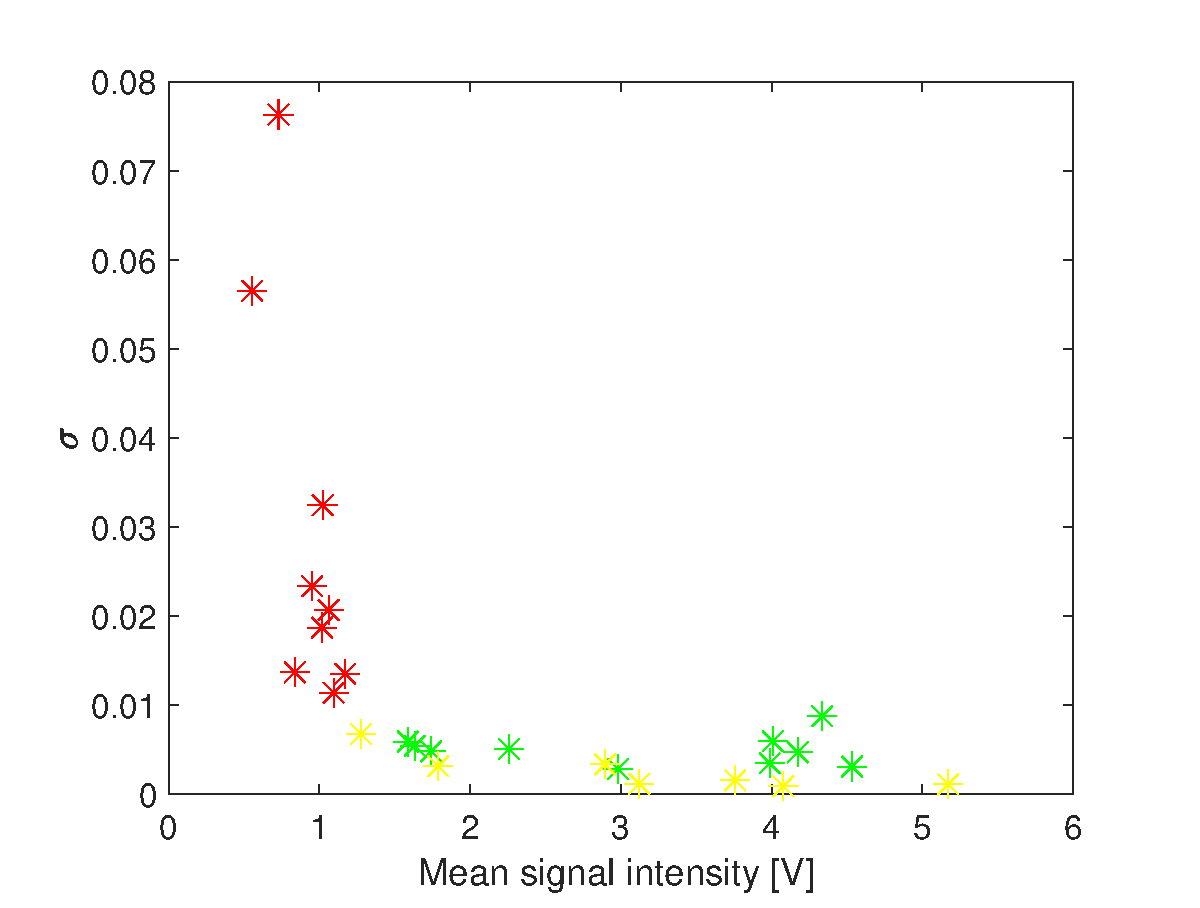
\includegraphics[width=1\textwidth]{result/noise/meanV_sigma.eps}
    \subcaption{}
    \label{fig:snr_v_sigma}
\end{minipage}
\begin{minipage}[t]{0.495\textwidth}
    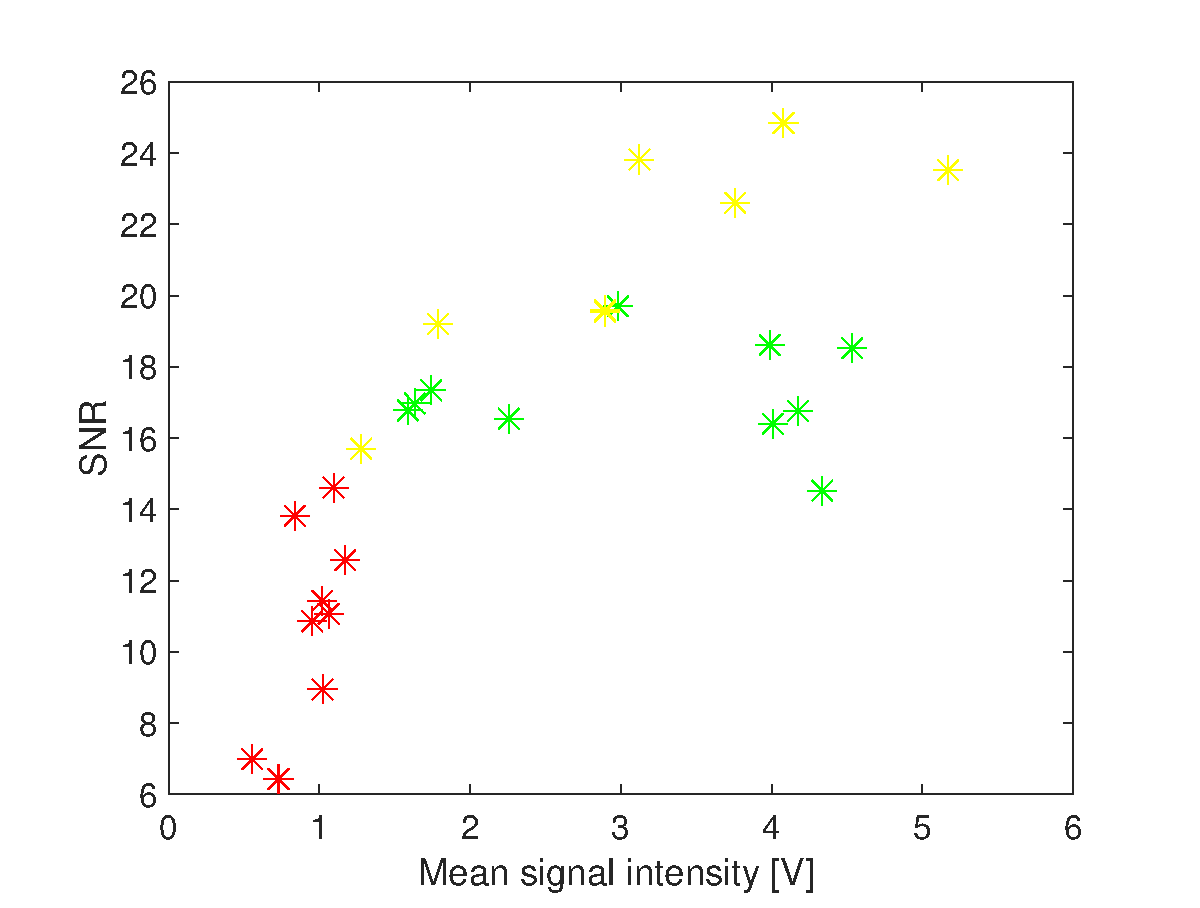
\includegraphics[width = \textwidth]{result/noise/meanV_snr.eps}
    \subcaption{}
    \label{fig:snr_v_SNR}
\end{minipage}
    \caption{Mean sampled signal intensity compared to normalized signal and background noise where each signal has the same corresponding color code from the BRISQUE plot in figure~\ref{fig:brisque_plot}.  (a) Signal intensity against normalized variance from background noise. (b) Signal intensity against SNR from normalized signal and background noise.}
    \label{fig:snr}
\end{figure}

From the two plots in figure~\ref{fig:snr} there are some conclusions that can be made:


\begin{itemize}
\item From both plots in figure~\ref{fig:snr} there is a quite distinct threshold where the signals intensity overcomes the noise level to reconstructed "good" images around 1.2 volt. None of the "good"/"half good" images are below this signal intensity but are mixed over the threshold. 
%The exponential characteristics of the signal to noise ratio given the signal strength means that it should be easy to find a threshold for a given systems background noise.

\item In the plots there are only two signals with higher variance than 0.04 which is the threshold where the the simulated images started to get both worse initial BRISQUE score and worse trend when increasing the subsampling ratio in figure~\ref{fig:Brisque_2d}. This implies that there must be at least one additional factor at play to reduce the image quality in the "bad" set. 


\item There are three red images with almost the same SNR and mean signal intensity as yellow and green images but yields a worse BRISQUE score anyway. This strengthening the statement the there is probably at least on more factor that reduces reconstruction performance.

\item The yellow and green images is mixed for all mean signal strengths which implies that the motive in the images effecting the  BRISQUE score. 

\end{itemize}

\todo[inline]{End klam}



\pagebreak

\subsubsection{Number of measurements}
From the theory of compressive sensing the number of measurements needed to reconstruct an image is correlated with the sparsity or compressibility of the image, therefore it is hard to give an exact  subsampling ratio needed. In this context the number of measurements needed refers to 

Using a SPC where noise contaminate the signal and the scene may not be completely stationary will increase the number of measurements needed. 


\begin{figure}[H]
\begin{minipage}[t]{0.3\linewidth} %Car
	\includegraphics[width = 1\linewidth]{gfx/car/car_org.png}
	\subcaption{Visual camera image.}
	\label{fig:car_org}
\end{minipage}
\begin{minipage}[t]{0.3\linewidth} % Hus
	\includegraphics[width = 1\linewidth]{gfx/hus/hus_org.png}
	\subcaption{}
	\label{fig:hus_org}
\end{minipage}
\begin{minipage}[t]{0.3\linewidth} %Sit
	\includegraphics[width = 1\linewidth]{gfx/sit/sit_org.png}
	\subcaption{}
	\label{fig:sit_org}
\end{minipage}
\begin{minipage}[t]{0.3\linewidth} %Car
	\includegraphics[width = 1\linewidth]{gfx/car/car_m5.png}
	\subcaption{Subsampling ratio 5\%}
	\label{fig:car_m5}
\end{minipage}
\begin{minipage}[t]{0.3\linewidth} % Hus
	\includegraphics[width = 1\linewidth]{gfx/hus/hus_m5.png}
	\subcaption{}
	\label{fig:hus_m5}
\end{minipage}
\begin{minipage}[t]{0.3\linewidth} %Sit
	\includegraphics[width = 1\linewidth]{gfx/sit/sit_m10.png}
	\subcaption{}
	\label{fig:sit_m5}
\end{minipage}
\begin{minipage}[t]{0.3\linewidth} %Car
	\includegraphics[width = 1\linewidth]{gfx/car/car_m10.png}
	\subcaption{Subsampling ratio 10\%}
	\label{fig:car_m10}
\end{minipage}
\begin{minipage}[t]{0.3\linewidth} % Hus
	\includegraphics[width = 1\linewidth]{gfx/hus/hus_m10.png}
	\subcaption{}
	\label{fig:hus_m10}
\end{minipage}
\begin{minipage}[t]{0.3\linewidth} %Sit
	\includegraphics[width = 1\linewidth]{gfx/sit/sit_m10.png}
	\subcaption{}
	\label{fig:sit_m10}
\end{minipage}
\end{figure}
\begin{figure}[H]
\ContinuedFloat
\begin{minipage}[t]{0.3\linewidth} %Car
	\includegraphics[width = 1\linewidth]{gfx/car/car_m15.png}
	\subcaption{Subsampling ratio 15\%}
	\label{fig:car_m15}
\end{minipage}
\begin{minipage}[t]{0.3\linewidth} % Hus
	\includegraphics[width = 1\linewidth]{gfx/hus/hus_m15.png}
	\subcaption{}
	\label{fig:hus_m15}
\end{minipage}
\begin{minipage}[t]{0.3\linewidth} %Sit
	\includegraphics[width = 1\linewidth]{gfx/sit/sit_m15.png}
	\subcaption{}
	\label{fig:sit_m15}
\end{minipage}
\begin{minipage}[t]{0.3\linewidth} %Car
	\includegraphics[width = 1\linewidth]{gfx/car/car_m20.png}
	\subcaption{Subsampling ratio 20\%}
	\label{fig:car_m20}
\end{minipage}
\begin{minipage}[t]{0.3\linewidth} % Hus
	\includegraphics[width = 1\linewidth]{gfx/hus/hus_m20.png}
	\subcaption{}
	\label{fig:hus_m20}
\end{minipage}
\begin{minipage}[t]{0.3\linewidth} %Sit
	\includegraphics[width = 1\linewidth]{gfx/sit/sit_m20.png}
	\subcaption{}
	\label{fig:sit_m20}
\end{minipage}
\begin{minipage}[t]{0.3\linewidth} %Car
	\includegraphics[width = 1\linewidth]{gfx/car/car_m25.png}
	\subcaption{Subsampling ratio 25\%}
	\label{fig:car_m25}
\end{minipage}
\begin{minipage}[t]{0.3\linewidth} % Hus
	\includegraphics[width = 1\linewidth]{gfx/hus/hus_m25.png}
	\subcaption{}
	\label{fig:hus_m25}
\end{minipage}
\begin{minipage}[t]{0.3\linewidth} %Sit
	\includegraphics[width = 1\linewidth]{gfx/sit/sit_m25.png}
	\subcaption{}
	\label{fig:sit_m25}
\end{minipage}
\begin{minipage}[t]{0.3\linewidth} %Car
	\includegraphics[width = 1\linewidth]{gfx/car/car_m30.png}
	\subcaption{Subsampling ratio 30\%}
	\label{fig:car_m30}
\end{minipage}
\begin{minipage}[t]{0.3\linewidth} % Hus
	\includegraphics[width = 1\linewidth]{gfx/hus/hus_m30.png}
	\subcaption{}
	\label{fig:hus_m30}
\end{minipage}
\begin{minipage}[t]{0.3\linewidth} %Sit
	\includegraphics[width = 1\linewidth]{gfx/sit/sit_m30.png}
	\subcaption{}
	\label{fig:sit_m30}
\end{minipage}
	\caption{Images reconstructed using $M/N = 5\% \text{ to } 30\%$ measurements from top down.} 
\end{figure}

\subsubsection{Soft chessboard}
\todo[inline]{Todo: Skapa rekonstruerade bilder från homagraphin och jämnför de rekonstruerade med referensbilden}
This evaluation is designed to confirm that the images reconstructed by the SPC follows the same characteristics as the reconstruction of the synthetic data.


\begin{figure}[H]
    \centering
\begin{minipage}[h]{0.3\textwidth}
	\vspace*{1cm}
    \includegraphics[width=1\textwidth]{result/hom/im_ref.png}
    \subcaption{Refrence image}
    \label{fig:hom_ref}
\end{minipage}
\begin{minipage}[t]{0.22\textwidth}
    \includegraphics[width = \textwidth]{result/hom/im_m5.png}
    \subcaption{5\%}
    \label{fig:hom_5}
    \includegraphics[width = \textwidth]{result/hom/im_m20.png}
    \subcaption{20\%}
    \label{fig:hom_20}
\end{minipage}
\begin{minipage}[t]{0.22\textwidth}
    \includegraphics[width = \textwidth]{result/hom/im_m10.png}
    \subcaption{10\%}
    \label{fig:hom_10}
    \includegraphics[width = \textwidth]{result/hom/im_m25.png}
    \subcaption{25\%}
    \label{fig:hom_25}
\end{minipage}
\begin{minipage}[t]{0.22\textwidth}
    \includegraphics[width = \textwidth]{result/hom/im_m15.png}
    \subcaption{15\%}
    \label{fig:hom_15}
    \includegraphics[width = \textwidth]{result/hom/im_m30.png}
    \subcaption{30\%}
    \label{fig:hom_30}
\end{minipage}

    \caption{The reconstructed images with different number of measurements and the reference image transformed to fit the SPC images using homography.}
    \label{fig:hom_over_im}
\end{figure}


\begin{figure}[H]
    \centering
\begin{minipage}[t]{0.49\textwidth}
    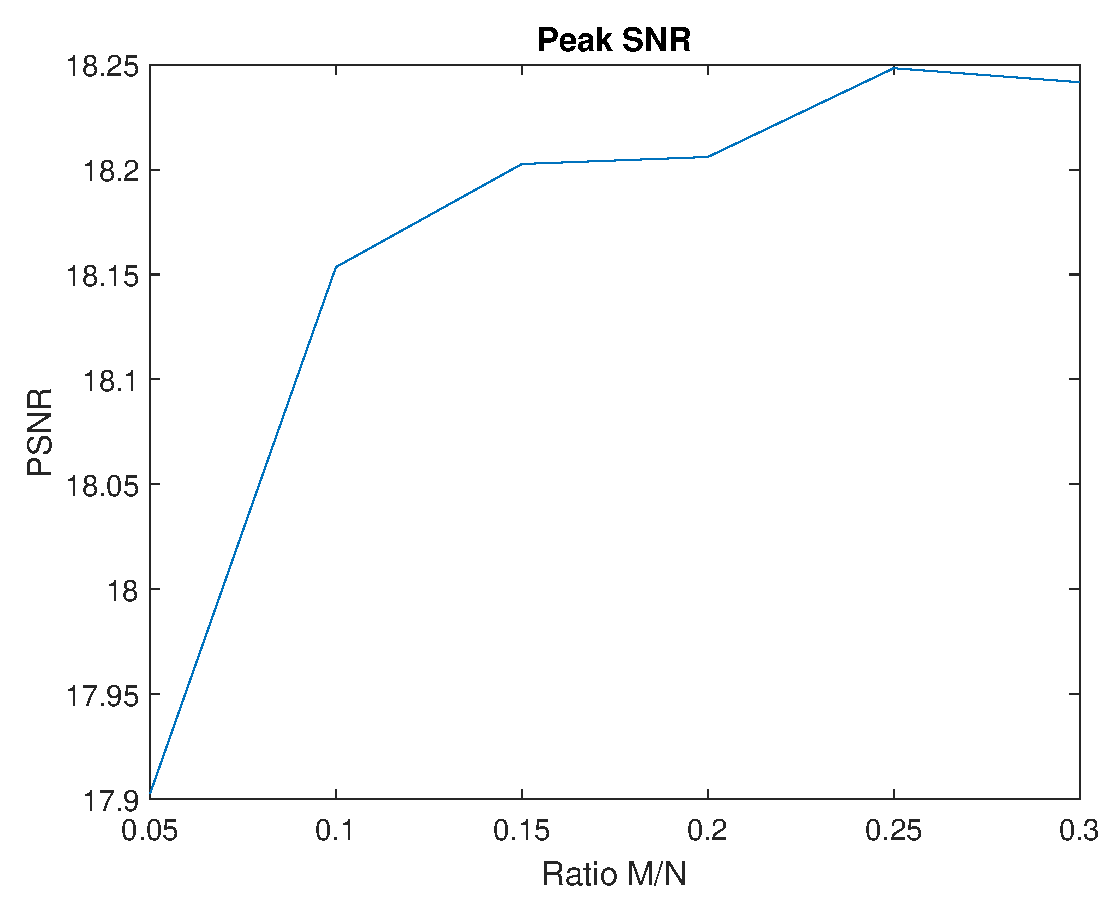
\includegraphics[width=1\textwidth]{result/homo/PSNR_2.eps}
    \subcaption{}
    \label{fig:hom_psnr}
\end{minipage}
\begin{minipage}[t]{0.49\textwidth}
    \includegraphics[width=1\textwidth]{result/homo/SSIM_2.eps}
    \subcaption{}
    \label{fig:hom_ssim}
\end{minipage}
    \caption{Signal quality of SPC images compared to reference image. (a) Peak SNR for reconstructed images against reference image. (b) SSIM score for reconstructed images against reference image.}
    \label{fig:hom_score}
\end{figure}





\subsubsection{Modulation Transfer Function}
The MTF is used to comparing the sharpness of cameras and lenses.  

%for two reasons: (1) Image contrast is half its low frequency or peak values,hence detail is still quite visible. The eye is relatively insensitive to detail at spatial frequencies where MTF is low: 10 or less. (2) The response of most cameras falls off rapidly in the vicinity of MTF50 and MTF50P. MTF50P is a better metric for strongly sharpened cameras that have “halos” near edges and corresponding peaks in their MTF response.

The MTF from the SPC is compared to a state of the art SWIR camera. Two scenes was captured by the SPC and a conventional SWIR camera containing printed sheath of paper with simple tilted shapes on them, see figure~\ref{fig:mtf_target}. 



\begin{figure}[H]
    \centering
    \includegraphics[width=0.9\linewidth]{result/mtf/Target.eps}
    \caption{Printed targets with markings where the MTF measurements was performed}
    \label{fig:mtf_target}
\end{figure}

\begin{figure}[H]
    \centering
\begin{minipage}[t]{0.45\textwidth}
    \includegraphics[width=1\textwidth]{result/mtf/swir2.png}
    \subcaption{}
    \label{fig:mtf_s2}
\end{minipage}
\begin{minipage}[t]{0.45\textwidth}
    \includegraphics[width=1\textwidth]{result/mtf/spc22.png}
    \subcaption{}
    \label{fig:mtf_spc2}
\end{minipage}
\begin{minipage}[t]{0.45\textwidth}
    \includegraphics[width=1\textwidth]{result/mtf/swir1.png}
    \subcaption{}
    \label{fig:mtf_s1}
\end{minipage}
\begin{minipage}[t]{0.45\textwidth}
    \includegraphics[width=1\textwidth]{result/mtf/spc12.png}
    \subcaption{}
    \label{fig:mtf_spc1}
\end{minipage}
    \caption{SPC and state of the art SWIR camera output images.}
    \label{fig:mtf_target_im}
\end{figure}

In the resulting images MTF measurements was performed on the specified edges to gather a mean and standard deviation for each camera. For the SPC, images reconstructed from 5\% to 30\% was tested in order to see if the number of measurements effected the MTF result. In figure~\ref{fig:mtf_target_im} the images from the SWIR camera and SPC are presented.



\todo[inline]{Light source 135W from 2m. Image on the board}


The edge response is measured in the distance (pixels) required for the edge to rise from $10\%$ to $90\%$. In figure~\ref{fig:rise} the result from the experiment in presented. 

\begin{figure}[H]
    \centering
    \includegraphics[width=0.7\linewidth]{result/mtf/Rise10_90.eps}
    \caption{10-90\% rise in pixels.}
    \label{fig:rise}
\end{figure}


\subsection{Luminance change in scene}
As predicted in section~\ref{sec:Dynamics_in_scene} dynamics in the scene could result in poor reconstruction performance.  

\begin{figure}[H]
\includegraphics[width = 0.7\linewidth]{result/luminance/li.eps}
	\caption{Sampled signal from SPC with light intensity change and the improved moving mean processed signal.}
	\label{fig:lc_plot}
\end{figure}


\begin{figure}[H]
\begin{minipage}[t]{0.49\textwidth}
\includegraphics[width = 1\linewidth]{result/luminance/24_512_m30.PNG}
	\subcaption{}
	\label{lc_bf}
\end{minipage}
\begin{minipage}[t]{0.49\textwidth}
\includegraphics[width = 1\linewidth]{gfx/car/car_m30.png}
	\subcaption{}
	\label{lc_af}
\end{minipage}
	\caption{Reconstructed images before and after applying moving mean average.}
	\label{fig:lc_image}
\end{figure}



\subsection{Noise analysis}
Volt to variance


